\documentclass[UTF8]{ctexart}

% ===== 基本宏包 =====
\usepackage{geometry}
\usepackage{titling}
\usepackage[nocompress]{cite}
\usepackage{graphicx}
\usepackage[perpage,stable]{footmisc}
\usepackage{amsmath}
\usepackage{amssymb, amsfonts}
\usepackage{float}
\usepackage{fancyhdr}
\usepackage{booktabs}
\usepackage{textcomp}
\usepackage{array}
\usepackage{tabularx}
\usepackage{multirow}
\usepackage{wasysym}
\usepackage{pifont}
\usepackage{subcaption}
\usepackage[ruled,vlined,linesnumbered,ruled]{algorithm2e}
\usepackage{titling} % 核心宏包，用于调整标题间距
\usepackage{hyperref}

\usepackage{url}
\usepackage{xcolor}
\makeatletter
\def\UrlFont{\color{blue}\ttfamily}
\makeatother

\newcommand{\cmark}{\ding{51}}      % 对号 ✓
\newcommand{\xmark}{\ding{55}}      % 错号 ✘
\newcommand{\tmark}{$\blacktriangle$} % 三角 ▲

% 2. 重定义maketitle，精准控制内部间距
\makeatletter
\renewcommand{\maketitle}{%
  \begin{center}
    \Large\bfseries \@title \\[10pt]
    \Large \@author \\[20pt]
    \small \@date
  \end{center}
  \vspace{-5pt}
}
\makeatother

\pagestyle{fancy}
\fancyhf{}                 % 清空默认页眉页脚
\fancyfoot[C]{\thepage}    % 页码放在底部中间
\renewcommand{\headrulewidth}{0pt} % 去掉页眉横线


\ctexset{
  section = {
    format = \raggedright\bfseries
  }
}


% ===== 页面设置 =====
\geometry{a4paper, left=2.5cm, right=2.5cm, top=2cm, bottom=2.5cm}
\begin{document}
\title{MPG-Former: Drift-Aware Multi-scale Prototype-Graph Transformer for Cloud Workload Forecasting}

\date{}

\maketitle

\section{引言}

\raggedright

云计算平台已经成为在线服务、批处理任务和数据密集型应用的核心运行基础\cite{ghemawat2003gfs,dean2004mapreduce,chang2006bigtable,decandia2007dynamo}。平台中的工作负载通常由 CPU 使用率、请求到达率、内存占用、任务执行量等连续监控序列刻画，并以大量实例、高采样频率和多租户共享环境的形式持续产生\cite{cortez2017resource,ousterhout2013sparrow,gog2016firmament}。为了避免资源过度预留造成浪费，或资源不足导致服务质量下降，云平台需要在负载真正到来之前完成扩缩容、容量规划和调度决策\cite{armbrust2009above,mell2011nist,hindman2011mesos,mao2019decima}。因此，准确的工作负载预测是弹性资源管理和 SLA 保障中的基础问题\cite{cortez2017resource,delimitrou2014quasar,zhang2021sinan}。近年来，长序列预测、频域建模和云负载预测方法不断提升模型对时间依赖、周期结构和典型负载模式的刻画能力\cite{zhou2021informer,wu2021autoformer,wang2023dyn,zhou2024fremer}。然而，真实云工作负载并不是一类平稳演化的普通时间序列，它由用户访问、应用调用链、调度策略、共址竞争、后台维护和多租户共享环境共同驱动，其局部运行状态会随时间持续变化\cite{cortez2017resource,delimitrou2013paragon,lo2015heracles,zhang2021sinan}。

现有预测范式通常将未来负载视为历史观测的时间延续，并默认某类主导证据在不同窗口中相对可靠\cite{lai2018lstnet,oreshkin2020nbeats,zhou2022fedformer}。例如，模型可以依赖近期时间记忆预测平稳片段，利用周期形态外推规律负载，或通过相似实例的同步变化补充跨序列信息。该假设在单一运行状态下往往有效，但在真实云平台中并不总是成立\cite{liu2022nonstationary,kim2021revin}。如图 \ref{fig:intro}(a) 所示，同一条工作负载在 $0$--$85$h 内主要在约 8--25 的低负载区间内周期振荡；进入 $86$--$157$h 后，负载虽然均值仅从约 16 上升到约 23，但局部峰值迅速增至 50 以上，表现为短时高负载突发；在 $158$--$259$h 内，负载均值进一步升至约 30，并伴随更高方差和整体水平上移，体现出漂移或非典型状态。与此同时，图 \ref{fig:intro}(b) 中三条工作负载虽然具有不同的绝对负载水平，但在约 55h、84h 和 101h 附近同时上升并随后回落，呈现明显的跨序列协同波动。

\begin{figure}[H]
    \centering
    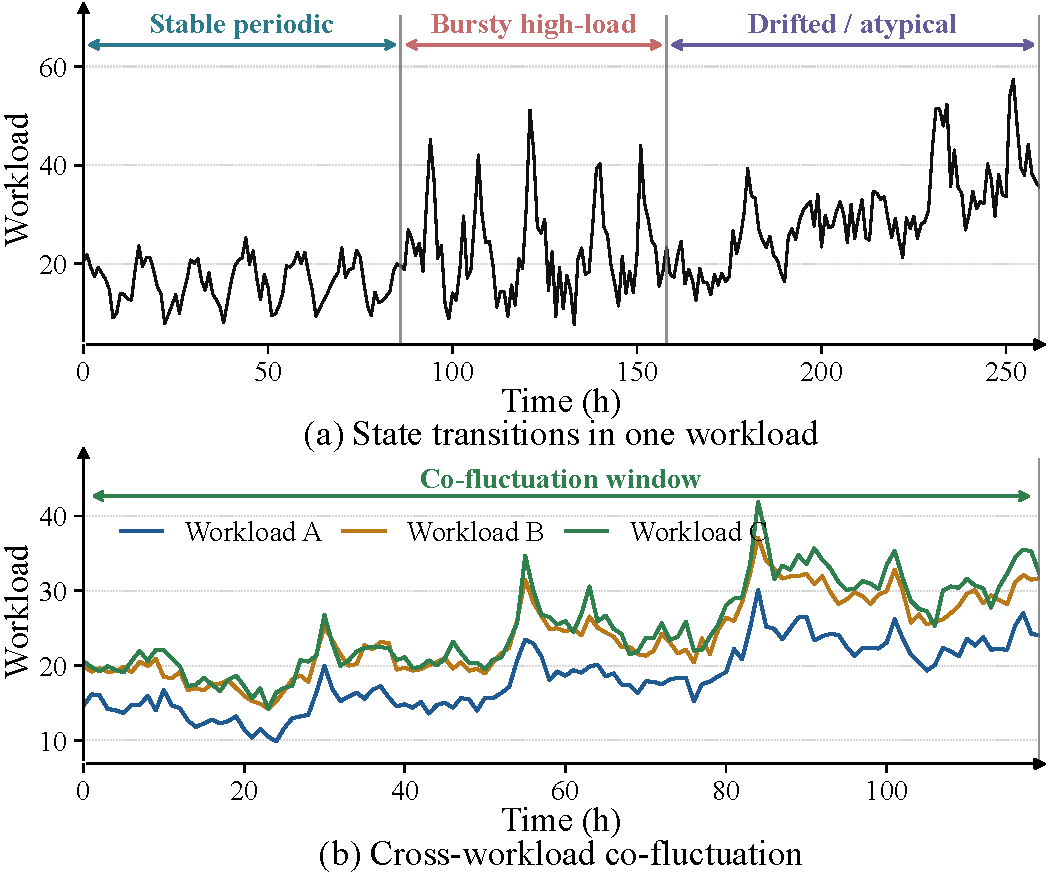
\includegraphics[width=0.5\columnwidth]{pic/intro.pdf}
    \caption{Representative workload states motivating evidence selection.}
    \label{fig:intro}
\end{figure}

这一观察暴露出云工作负载预测中的三个核心限制。

\textbf{L1: 窗口级非平稳动态.} 图 \ref{fig:intro}(a) 中的同一条序列在三个时间段内呈现出不同统计特征：稳定段的波动范围较窄，突发段的峰值约为稳定段峰值的两倍，漂移段的平均水平明显高于前两个阶段。模型在进入预测窗口之前并不知道当前片段属于哪一种状态。若缺乏窗口级状态感知，固定的时间依赖容易在稳定片段中过度响应噪声，在突发片段中低估峰值幅度，在漂移片段中继续沿用已经失效的历史尺度。

\textbf{L2: 多尺度形态混合.} 云负载的局部尖峰、短期抖动、批任务启动和周期性维护对应不同持续时间与频谱特征。图 \ref{fig:intro}(a) 中，稳定段需要观察几十小时才能辨识其重复节律，而突发段的高峰通常只在数小时内完成上升和回落；漂移段又表现为更长时间尺度上的基线抬升。单一尺度表示难以同时描述短时尖峰、周期振荡和长期漂移，也难以判断当前窗口是否仍符合历史中常见的典型模式。

\textbf{L3: 窗口相关的跨序列关系.} 图 \ref{fig:intro}(b) 表明，不同工作负载虽然基线水平不同，但在若干局部窗口内具有相似的升降方向。例如在约 84h 附近，三条序列同时达到局部高峰，说明相似服务逻辑、共享流量、共址资源竞争或调度事件可能在短时间内形成有效的跨序列参考。但这种协同关系通常只在特定窗口内出现，并不等价于长期固定拓扑。若始终使用静态邻居，模型可能在协同窗口中遗漏有效参考，也可能在非协同窗口中引入无关噪声。

因此，云工作负载预测更适合被建模为一个状态依赖的证据选择问题。稳定窗口应更多依赖时间记忆和典型周期，突发窗口应强调局部短期变化，协同窗口需要引入相似负载的跨序列信息，而漂移窗口则应降低对历史模式的盲目外推。虽然已有方法能够从时间依赖、频率结构、全局模式或图关系等角度提升预测性能，但它们通常围绕某一种主要信息源构建预测过程，缺少在样本级别重新分配预测证据的显式机制。当负载状态在不同窗口之间切换时，这种固定证据假设会限制模型对复杂云环境的适应能力。

为此，本文提出 MPG-Former，一个面向云工作负载预测的漂移感知多证据框架。MPG-Former 同时构造三类互补证据：时间证据刻画目标实例自身历史，多尺度时频原型证据检索典型负载形态，动态图证据捕获当前批内临时协同关系。针对 L1，模型利用窗口统计量调制时间证据建模过程，使注意力能够适应局部非平稳状态；针对 L2，模型将多尺度时域片段与频域幅值映射到可学习原型记忆中，以评估当前形态与典型模式的匹配程度；针对 L3，模型在小批量内动态构建负载图和上下文图，从相似窗口中聚合跨序列证据。最后，漂移感知路由器根据窗口漂移特征和原型不确定性为三类证据分配样本级权重，并生成未来负载预测。

本文的主要贡献如下：
\begin{enumerate}
    \item 本文从状态依赖证据选择角度重新审视云工作负载预测，指出不同运行窗口对时间证据、原型证据和图证据的依赖会动态变化。
    \item 本文设计 MPG-Former，将非平稳时间建模、多尺度时频原型检索和批内动态图证据统一到一个漂移感知预测框架中。
    \item 本文提出漂移感知路由机制，根据窗口统计变化与原型不确定性自适应融合多类证据，从而增强模型对周期、突发、协同和漂移状态的适应能力。
    \item 本文在多个云工作负载数据集上进行系统实验，验证 MPG-Former 在预测精度、组件有效性、参数敏感性、计算效率和证据选择可解释性方面的优势。
\end{enumerate}

\section{相关工作}

\noindent\textbf{时间序列预测.}
时间序列预测旨在从历史观测中推断未来变化，是资源调度、异常预警和容量规划中的基础任务。近年来，Transformer 结构被广泛用于长序列预测。Informer 通过稀疏注意力降低长序列建模复杂度\cite{zhou2021informer}，Autoformer 将序列分解与自相关机制结合以刻画趋势和周期\cite{wu2021autoformer}，Non-stationary Transformer 进一步引入去平稳化机制以缓解局部分布变化\cite{liu2022nonstationary}。此外，PatchTST 将时间序列划分为 patch 并采用通道独立建模\cite{nie2023patchtst}，iTransformer 则通过反转时间点和变量维度增强多变量交互建模\cite{liu2024itransformer}。这些方法提升了长序列依赖建模能力，但通常将预测过程视为统一的时间映射，较少显式刻画不同窗口中主导证据的变化。

\noindent\textbf{频域与多尺度建模.}
周期结构、频域特征和多尺度上下文能够揭示时间序列中的长期规律。PDF 通过周期解耦对不同周期模式进行分离\cite{dai2024pdf}，MICN 采用多尺度卷积同时捕获局部和全局上下文\cite{wang2023micn}，SOFTS 通过序列核心融合建模多变量序列之间的交互\cite{han2024softs}。这类方法说明，复杂序列往往需要从多个时间尺度或频率视角进行表示。然而，云负载中的周期形态并不总是稳定可靠，突发峰值和漂移状态可能使当前窗口偏离历史周期。MPG-Former 因此不仅提取多尺度时频特征，还将其组织为可学习原型记忆，并使用原型响应和不确定性衡量当前窗口与典型模式的匹配程度。

\noindent\textbf{图结构时间序列建模.}
将时间序列建模为图可以刻画变量、传感器或实例之间的依赖关系。早期图时序模型通常依赖预定义拓扑，例如 DCRNN 使用扩散卷积和循环结构建模交通网络中的时空传播\cite{li2018dcrnn}，STGCN 结合图卷积与时间卷积捕获空间和时间依赖\cite{yu2018stgcn}。为缓解固定图结构的限制，Graph WaveNet 引入自适应邻接矩阵以学习潜在依赖\cite{wu2019graphwavenet}。这些方法表明图关系对多变量预测具有重要价值。不同的是，云工作负载中的协同关系往往是窗口相关且短暂出现的，难以由静态拓扑完全描述。MPG-Former 在小批量内动态构建负载相似图和上下文相似图，并将图表示作为一种候选预测证据参与路由。

\noindent\textbf{云工作负载预测.}
云工作负载预测面向多租户共享、应用变化和资源竞争等生产环境特征。DynEformer 面向动态多租户边缘云平台，通过全局模式池和动态信息融合实现统一工作负载预测\cite{wang2023dyn}；Fremer 将轻量频率 Transformer 用于云服务负载预测，以捕获云负载中的频域规律\cite{zhou2024fremer}；TFEGRU 结合时频增强和门控循环结构刻画云负载变化\cite{tfegru2024}。这些工作从全局模式、频率结构或时频增强角度提升了云场景预测性能。MPG-Former 进一步关注同一实例在正常运行过程中预测证据来源的动态切换，将时间证据、原型证据和动态图证据统一到漂移感知证据选择框架中。

\section{问题定义}

考虑一个由 $N$ 条云工作负载序列组成的数据集 $\mathcal D=\{(\mathbf X_i,\mathbf s_i)\}_{i=1}^{N}$。其中，$\mathbf X_i\in\mathbb R^{T_i\times C}$ 表示第 $i$ 个对象在 $T_i$ 个时间戳上的 $C$ 维动态观测，$\mathbf s_i\in\mathbb R^{C_s}$ 表示可选的静态上下文。给定目标通道索引 $c_0$，目标工作负载记为 $y_{i,t}=\mathbf X_{i,t,c_0}$。若静态上下文不可用，则 $\mathbf s_i$ 记为空向量。该定义不限定具体数据来源、采样间隔或通道语义，只要求目标通道为待预测的工作负载序列。

给定历史长度 $L$ 和预测长度 $H$，每条长序列被切分为因果滑动窗口。对于第 $i$ 条序列在时刻 $t$ 的窗口，历史输入和未来监督目标分别定义为
\begin{equation}
    \mathbf X^{h}_{i,t}=\mathbf X_{i,t-L+1:t,:}\in\mathbb R^{L\times C},\quad
    \mathbf y^{f}_{i,t}=[y_{i,t+1},\ldots,y_{i,t+H}]\in\mathbb R^{H}.
    \label{eq:window_problem}
\end{equation}
式 \eqref{eq:window_problem} 保证预测目标严格位于历史窗口之后。因此，在训练和推理中，模型只能利用 $\mathbf X^{h}_{i,t}$ 及其对应的可用上下文 $\mathbf s_i$ 来预测未来目标负载 $\mathbf y^{f}_{i,t}$，不能访问未来真实目标值。

为与后续方法描述保持一致，本文以包含 $B$ 个窗口的小批量作为基本计算单位。将历史窗口堆叠后，记编码器历史输入为 $\mathbf X^{enc}\in\mathbb R^{B\times L\times C}$，目标历史通道为 $\mathbf x^{hist}=\mathbf X^{enc}_{:,:,c_0}\in\mathbb R^{B\times L}$，对应静态上下文为 $\mathbf s\in\mathbb R^{B\times C_s}$。其中 $B$ 表示批量大小，$\mathbf x^{hist}$ 是目标通道在历史窗口内的观测矩阵，后续模型描述均采用上述批量记号。

本文的预测任务是学习一个参数化函数 $F_{\theta}$，使其根据历史窗口和可用上下文输出未来 $H$ 个时间点的目标负载：
\begin{equation}
    \hat{\mathbf y}_{i,t}=F_{\theta}(\mathbf X^{h}_{i,t},\mathbf s_i)\in\mathbb R^H.
    \label{eq:forecast_problem}
\end{equation}
模型参数通过最小化预测误差风险获得：
\begin{equation}
    \theta^{*}=\arg\min_{\theta}\mathbb E_{(i,t)}\left[\mathcal L_{err}(\hat{\mathbf y}_{i,t},\mathbf y^{f}_{i,t})\right].
    \label{eq:objective_problem}
\end{equation}
其中 $\mathcal L_{err}$ 表示预测误差损失，$\mathbb E_{(i,t)}[\cdot]$ 表示对所有可用窗口的经验期望。式 \eqref{eq:forecast_problem}--\eqref{eq:objective_problem} 构成本文所研究的云工作负载多步预测问题。

\section{方法}

\begin{figure}[t]
    \centering
    \includegraphics[width=\textwidth]{pic/architecture.pdf}
    \caption{Overall architecture of MPG-Former.}
    \label{fig:architecture}
\end{figure}

图 \ref{fig:architecture} 展示了 MPG-Former 的整体框架。
整体而言，MPG-Former 由以下五个主要模块组成：
\begin{itemize}
    \item \textbf{输入构造与历史表示生成}，将原始窗口分解为历史编码器输入和未来解码器输入，并将归一化后的多通道历史映射到统一隐藏空间（Section \ref{sec:history_representation}）。
    \item \textbf{非平稳时间证据建模}，使用窗口统计量调制自注意力，并结合趋势--残差分解与短期时序编码器提取目标实例自身历史证据（Section \ref{sec:temporal_evidence}）。
    \item \textbf{多尺度时频原型检索}，在多个时间尺度上联合建模时域片段和频域幅值，并从可学习原型记忆中检索典型负载形态（Section \ref{sec:prototype_evidence}）。
    \item \textbf{动态图证据建模}，在当前小批量内根据负载相似性和上下文相似性动态构图，并通过图消息传递获得跨序列证据（Section \ref{sec:graph_evidence}）。
    \item \textbf{漂移感知融合与解码}，依据漂移特征和原型不确定性自适应融合三类证据，并输出点预测、区间预测和可解释权重（Section \ref{sec:fusion_decoding}）。
\end{itemize}

\subsection{目标通道归一化与历史表示生成}
\label{sec:history_representation}

如图 \ref{fig:architecture}(a) 所示，本节介绍 MPG-Former 如何从原始负载窗口构造编码器/解码器输入，并生成后续证据分支共享的历史表示。

\noindent\textbf{目标通道归一化.}
云工作负载在不同实例、不同应用和不同时间段上具有明显尺度差异。直接在原始尺度上学习会使模型过度关注绝对量级，而忽略窗口内部的形态变化。因此，MPG-Former 仅对目标通道执行窗口级可逆归一化，其他动态协变量保持原始相对结构。给定小批量中的历史目标窗口 $\mathbf x^{hist}$，第 $b$ 个样本的均值和标准差分别记为 $\mu_b=\frac{1}{L}\sum_{t=1}^{L}x^{hist}_{b,t}$ 和 $\sigma_b=\max\{\sqrt{\frac{1}{L}\sum_{t=1}^{L}(x^{hist}_{b,t}-\mu_b)^2},\epsilon\}$，归一化目标历史为
\begin{equation}
    \tilde{x}^{hist}_{b,t}=\frac{x^{hist}_{b,t}-\mu_b}{\sigma_b}.
    \label{eq:mpg_target_norm_new}
\end{equation}
其中 $\epsilon$ 为数值稳定项。归一化后的目标通道被替换回编码器输入，形成 $\tilde{\mathbf X}^{enc}$。式 \eqref{eq:mpg_target_norm_new} 中的 $\mu_b$ 和 $\sigma_b$ 会被保存，并在式 \eqref{eq:mpg_prediction_new} 中用于将归一化空间预测恢复到原始负载尺度。这样，模型中间表示在局部尺度上更加稳定，而最终评价仍在原始工作负载尺度上完成。

\noindent\textbf{历史表示生成.}
给定解码器历史标签长度 $\ell$，MPG-Former 使用前 $L$ 个时间点作为编码器输入，并使用最后 $\ell$ 个历史点与 $H$ 个未来掩码位置构造解码器输入。令 $d_m$ 表示隐藏维度，$\mathbf W_{in}\in\mathbb R^{C\times d_m}$ 为输入投影矩阵，$\mathbf{PE}\in\mathbb R^{L\times d_m}$ 为位置编码，则归一化编码器输入首先被映射为 $\mathbf Z_0=\tilde{\mathbf X}^{enc}\mathbf W_{in}+\mathbf{PE}$。当静态上下文 $\mathbf s\in\mathbb R^{B\times C_s}$ 可用时，模型通过门控静态融合为每个时间位置注入实例、应用或机器级先验：令 $\mathbf a_t=\operatorname{softmax}(\mathbf z_{0,t}\mathbf W_q^{s})$ 和 $\mathbf v_s=\mathbf s\mathbf W_v^{s}$，其中 $\mathbf W_q^{s}$ 与 $\mathbf W_v^{s}$ 为可学习映射；第 $t$ 个历史表示被更新为 $\operatorname{LayerNorm}(\mathbf z_{0,t}+\mathbf a_t\odot\mathbf v_s)$。该过程记为
\begin{equation}
    \mathbf H_s=\operatorname{StaticGate}(\tilde{\mathbf X}^{enc}\mathbf W_{in}+\mathbf{PE},\mathbf s).
    \label{eq:mpg_history_repr_new}
\end{equation}
其中 $\operatorname{StaticGate}$ 表示静态上下文门控和层归一化；若静态上下文缺失，该操作退化为恒等映射。输出 $\mathbf H_s\in\mathbb R^{B\times L\times d_m}$ 是后续所有证据分支的历史基础，时间分支以 $\mathbf X_1=\mathbf H_s$ 作为第一层输入。

\subsection{非平稳时间证据建模}
\label{sec:temporal_evidence}

如图 \ref{fig:architecture}(b) 所示，本节介绍非平稳时间证据分支如何利用窗口统计量调制注意力，并进一步结合趋势--残差分解和短期时序编码获得时间证据。

\noindent\textbf{统计调制的自注意力.}
时间证据分支刻画目标实例自身历史对未来负载的解释能力。由于同一条云负载序列可能在稳定周期、突发峰值和局部漂移之间切换，固定注意力温度难以适应不同窗口状态。MPG-Former 因此使用归一化目标历史的窗口统计量调制每一层注意力。对于第 $b$ 个样本，统计向量定义为 $\mathbf s^{stat}_b=[\operatorname{mean}(\tilde{\mathbf x}^{hist}_b),\operatorname{std}(\tilde{\mathbf x}^{hist}_b)]$，并通过统计调制器生成注意力温度和偏置：
\begin{equation}
    [\boldsymbol{\rho}_b,\boldsymbol{\delta}_b]=\operatorname{MLP}_{stat}(\mathbf s^{stat}_b).
    \label{eq:mpg_stat_control_new}
\end{equation}
其中 $\boldsymbol{\tau}_b=\operatorname{softplus}(\boldsymbol{\rho}_b)+\epsilon_{\tau}$ 为正的注意力温度，$\boldsymbol{\delta}_b$ 为注意力偏置，二者均按注意力头生成。给定第 $l$ 层输入 $\mathbf X_l\in\mathbb R^{B\times L\times d_m}$，且 $\mathbf X_1=\mathbf H_s$，联合线性映射 $[\mathbf Q_l,\mathbf K_l,\mathbf V_l]=\operatorname{Split}(\mathbf X_l\mathbf W_{qkv}^{(l)})$ 产生查询、键和值，其中 $\mathbf W_{qkv}^{(l)}\in\mathbb R^{d_m\times 3d_m}$ 为第 $l$ 层可学习投影矩阵。若注意力头数为 $h$，单头维度为 $d_h=d_m/h$，则窗口调制后的注意力权重为
\begin{equation}
    \mathbf A_l=\operatorname{softmax}\!\left(\boldsymbol{\tau}_b\odot\frac{\mathbf Q_l\mathbf K_l^{\top}}{\sqrt{d_h}}+\boldsymbol{\delta}_b\right).
    \label{eq:mpg_ns_attention_new}
\end{equation}
式 \eqref{eq:mpg_ns_attention_new} 中的 $\mathbf A_l$ 与 $\mathbf V_l$ 加权得到注意力上下文 $\mathbf O_l=(\mathbf A_l\mathbf V_l)\mathbf W_o$，其中 $\mathbf W_o\in\mathbb R^{d_m\times d_m}$ 为输出投影。温度 $\boldsymbol{\tau}_b$ 控制历史位置之间依赖分布的尖锐程度，偏置 $\boldsymbol{\delta}_b$ 则为当前窗口提供样本级注意力平移，因此同一层可根据窗口状态改变时间聚合方式。

\noindent\textbf{趋势--残差更新.}
仅依赖注意力容易混合平滑趋势和短时尖峰。为此，每层同时对 $\mathbf X_l$ 执行移动平均分解：趋势项为 $\mathbf T_l=\operatorname{MA}_{k_{ma}}(\mathbf X_l)=\operatorname{AvgPool1D}(\operatorname{Pad}(\mathbf X_l),k_{ma})$，残差项为 $\mathbf S_l=\mathbf X_l-\mathbf T_l$。其中 $\operatorname{Pad}$ 表示边界填充，$k_{ma}$ 为移动平均核大小。趋势项提供低频演化方向，残差项保留突发和短期振荡。模型先将注意力上下文和趋势残差注入为 $\mathbf U_l=\operatorname{LayerNorm}(\mathbf X_l+\operatorname{Dropout}(\mathbf O_l)+0.1\mathbf T_l)$，再通过 $\mathbf X_{l+1}=\operatorname{LayerNorm}(\mathbf U_l+\operatorname{Dropout}(\operatorname{FFN}(\mathbf S_l+\mathbf U_l)))$ 生成下一层表示。因此，$\mathbf A_l$、$\mathbf T_l$ 和 $\mathbf S_l$ 分别承担长程依赖、平滑趋势和局部扰动建模。

\noindent\textbf{短期时间编码.}
经过 $e$ 层非平稳注意力后得到 $\mathbf X_{e+1}$。为了增强对突发窗口和短邻域形态的响应，MPG-Former 进一步使用短期时序编码器：$\mathbf C_{\mathrm{loc}}=\tanh(\operatorname{Conv}_{3}(\mathbf X_{e+1}))+\tanh(\operatorname{Conv}_{5}(\mathbf X_{e+1}))$ 捕获不同局部尺度的卷积模式，$\mathbf R_{\mathrm{gru}}=\operatorname{BiGRU}(\mathbf X_{e+1})$ 捕获顺序依赖。二者拼接后经线性映射和残差归一化得到 $\mathbf X_E=\operatorname{LayerNorm}(\mathbf X_{e+1}+\operatorname{Dropout}(\operatorname{Linear}([\mathbf C_{\mathrm{loc}};\mathbf R_{\mathrm{gru}}])))$。时间证据向量由 $\mathbf X_E$ 池化得到：
\begin{equation}
    \mathbf c_{time}=\frac{1}{L}\sum_{t=1}^{L}(\mathbf X_E)_{:,t,:}.
    \label{eq:mpg_time_context_new}
\end{equation}
其中 $\mathbf c_{time}\in\mathbb R^{B\times d_m}$ 进入动态图分支和路由器；逐时间点表示 $\mathbf X_E\in\mathbb R^{B\times L\times d_m}$ 则作为式 \eqref{eq:mpg_decoder_new} 中解码器记忆的主体。

\subsection{多尺度时频原型检索}
\label{sec:prototype_evidence}

如图 \ref{fig:architecture}(c) 所示，本节介绍多尺度时频原型分支如何从目标历史中构造尺度级表示，并通过原型记忆检索可复用的典型负载形态。

\noindent\textbf{尺度级时频 token.}
云工作负载中常见的日周期、批任务启动和短时冲高等形态通常在不同时间尺度上出现。多尺度时频原型分支的目标是学习这些可复用形态，并在预测时检索与当前窗口最相似的典型模式。给定归一化目标历史 $\tilde{\mathbf x}^{hist}$，模型使用尺度集合 $\mathcal P=\{6,12,24,48\}$ 进行非重叠切分。对于尺度 $p$，$\mathbf P_p=\operatorname{Unfold}(\tilde{\mathbf x}^{hist},p,p)\in\mathbb R^{B\times n_p\times p}$，其中 $n_p=L/p$。时域 token 由每个片段线性映射后在片段维平均得到，频域 token 则由每个片段的实值 FFT 幅值映射后平均得到。二者相加并经非线性函数形成尺度表示：
\begin{equation}
    \mathbf z_p=\tanh(\mathbf z^{time}_p+\mathbf z^{freq}_p).
    \label{eq:mpg_scale_token_new}
\end{equation}
其中 $\mathbf z^{time}_p=\operatorname{mean}_{j}(\mathbf P_{p,j}\mathbf W^{time}_p)$，$\mathbf z^{freq}_p=\operatorname{mean}_{j}(|\operatorname{rFFT}(\mathbf P_{p,j})|\mathbf W^{freq}_p)$；$\mathbf W^{time}_p$ 和 $\mathbf W^{freq}_p$ 为尺度 $p$ 的可学习投影矩阵。$\mathbf z_p$ 同时表示该尺度下的局部形态和频谱能量。尺度权重由 $\alpha_p=\operatorname{softmax}_{p}(\mathbf w_{\alpha}^{\top}\mathbf z_p)$ 得到，并在式 \eqref{eq:mpg_proto_context_new} 中控制不同尺度响应的占比。

\noindent\textbf{原型匹配与恢复.}
设可学习原型记忆为 $\mathbf M\in\mathbb R^{|\mathcal P|\times K\times d_m}$，每个尺度维护 $K$ 个原型。尺度表示与同尺度原型进行软匹配：
\begin{equation}
    \boldsymbol{\beta}_{p}=\operatorname{softmax}\!\left((\mathbf z_p\mathbf W_q)\mathbf M_p^{\top}/\sqrt{d_m}\right).
    \label{eq:mpg_proto_weight_new}
\end{equation}
其中 $\mathbf M_p\in\mathbb R^{K\times d_m}$ 为尺度 $p$ 的原型矩阵，$\mathbf W_q\in\mathbb R^{d_m\times d_m}$ 为共享查询投影。$\boldsymbol{\beta}_{p}$ 在 $K$ 个原型上归一化，表示当前窗口对同尺度原型的软分配。模型根据 $\boldsymbol{\beta}_{p}$ 读取原型响应 $\mathbf r_p=\boldsymbol{\beta}_{p}\mathbf M_p$，并通过恢复模块得到 $\hat{\mathbf r}_p=\operatorname{Recover}(\mathbf r_p+\mathbf z_p)$。其中 $\operatorname{Recover}$ 由层归一化、线性映射、GELU 和 Dropout 组成，用于将检索到的原型与当前尺度表示重新对齐。最终，四个尺度被融合为原型证据：
\begin{equation}
    \mathbf c_{proto}=\sum_{p\in\mathcal P}\alpha_p\hat{\mathbf r}_p.
    \label{eq:mpg_proto_context_new}
\end{equation}
原型上下文 $\mathbf c_{proto}$ 具有两种下游作用：其一，它作为原型证据进入路由器；其二，它被线性映射为未来目标通道的初始填充 $\mathbf p_{fut}=\mathbf c_{proto}\mathbf W_f+\mathbf b_f$，其中 $\mathbf W_f\in\mathbb R^{d_m\times H}$ 和 $\mathbf b_f\in\mathbb R^{H}$ 为可学习参数，并在式 \eqref{eq:mpg_decoder_new} 之前写入解码器未来位置。模型还将 $\alpha_p\boldsymbol{\beta}_p$ 展平为原型匹配分布 $\boldsymbol{\pi}$，并计算归一化熵 $\mathcal H_{proto,b}=-\sum_j \pi_{b,j}\log\pi_{b,j}/\log(|\mathcal P|K)$，用于衡量当前窗口与已学习原型之间的不确定性。

\subsection{动态图证据建模}
\label{sec:graph_evidence}

如图 \ref{fig:architecture}(d) 所示，本节介绍动态图证据分支如何在当前小批量内构建负载相似图和上下文相似图，并通过图消息传递提取跨序列证据。

\noindent\textbf{批内动态关系构建.}
云平台中的实例并非孤立运行。共同上游流量、调度批次或资源竞争会导致不同工作负载在局部窗口内出现协同波动。MPG-Former 将小批量中的每个样本窗口视为一个节点，并分别构建负载相似图和上下文相似图。负载相似图使用归一化目标历史作为节点特征 $\mathbf u^w_b=\tilde{\mathbf x}^{hist}_b$；上下文相似图优先使用静态上下文投影 $\mathbf u^c_b=\mathbf s_b\mathbf W_{ctx}$。若无静态特征，则使用窗口状态统计 $\mathbf r_b=[\operatorname{mean}(\tilde{\mathbf x}^{hist}_b),\operatorname{std}(\tilde{\mathbf x}^{hist}_b),\operatorname{mean}(|\Delta \tilde{\mathbf x}^{hist}_b|),\tilde{x}^{hist}_{b,L}-\tilde{x}^{hist}_{b,1}]$ 并投影为 $\mathbf u^c_b=\mathbf r_b\mathbf W_{state}$。给定任意一类节点特征 $\mathbf u_b$，邻接矩阵通过非负余弦相似度、Top-$k_{nn}$ 稀疏化和行归一化构造：
\begin{equation}
    \mathbf A=\operatorname{RowNorm}\!\left(\operatorname{TopK}_{k_{nn}}(\operatorname{ReLU}(\operatorname{Cos}(\mathbf u_b,\mathbf u_j)))+\mathbf I\right).
    \label{eq:mpg_adj_new}
\end{equation}
其中 $\operatorname{Cos}$ 为余弦相似度，$\mathbf I$ 为自环矩阵。由 $\mathbf u^w$ 和 $\mathbf u^c$ 分别得到 $\mathbf A^w$ 和 $\mathbf A^c$。Top-$k_{nn}$ 稀疏化使每个节点只从少量相似窗口接收信息，自环则保证节点自身表示不会在聚合中丢失。

\noindent\textbf{图消息传递与视角对齐.}
动态图分支以时间证据矩阵 $\mathbf C_{time}\in\mathbb R^{B\times d_m}$ 为节点初始表示。对于关系类型 $r\in\{w,c\}$，图卷积先执行邻居聚合 $\mathbf G^r=\mathbf A^r\mathbf C_{time}$，再得到残差更新 $\mathbf Z^r=\operatorname{LayerNorm}(\mathbf C_{time}+\operatorname{Dropout}(\operatorname{GELU}(\mathbf G^r\mathbf W_g^r)))$。其中 $\mathbf Z^w$ 和 $\mathbf Z^c$ 分别表示负载相似图与上下文相似图传播后的节点表示。二者被拼接并投影为图证据：
\begin{equation}
    \mathbf c_{graph}=\operatorname{LayerNorm}\!\left(\operatorname{GELU}(\operatorname{Linear}([\mathbf Z^{w};\mathbf Z^{c}]))\right).
    \label{eq:mpg_graph_context_new}
\end{equation}
为了使两种图视角形成一致而互补的跨序列表示，模型使用小批量内对比约束：
\begin{equation}
    \mathcal L_{con}=\operatorname{InfoNCE}(\mathbf Z^{w},\mathbf Z^{c}).
    \label{eq:mpg_contrast_new}
\end{equation}
具体而言，$\operatorname{InfoNCE}$ 将同一窗口在两种图中的表示作为正样本，将其他窗口作为负样本，并以温度 $T_c$ 计算双向交叉熵。该损失会在式 \eqref{eq:mpg_training_loss_new} 中参与优化，使图证据不仅来自相似邻居的聚合，也受到跨视角一致性的约束。

\subsection{漂移感知融合、解码与训练}
\label{sec:fusion_decoding}

如图 \ref{fig:architecture}(e) 所示，本节介绍 MPG-Former 如何根据窗口漂移状态融合三类证据，并利用增强解码记忆生成未来工作负载预测。

\noindent\textbf{漂移感知证据路由.}
时间证据、图证据和原型证据并不存在全局固定的优先级。稳定周期窗口通常更依赖原型记忆，突发或漂移窗口更需要近期时间证据，而协同波动窗口则更依赖图证据。MPG-Former 因此从归一化目标历史和原型匹配分布中提取漂移特征。对于第 $b$ 个样本，漂移向量为 $\mathbf d_b=[|\tilde{x}^{hist}_{b,L}-\operatorname{mean}(\tilde{\mathbf x}^{hist}_b)|/\operatorname{std}(\tilde{\mathbf x}^{hist}_b),\operatorname{mean}(|\Delta\tilde{\mathbf x}^{hist}_b|),\operatorname{std}(\tilde{\mathbf x}^{hist}_b),\mathcal H_{proto,b}]$，其中前三项刻画末端偏离、近期变化幅度和窗口波动强度，最后一项为原型不确定性。漂移分数由 $\kappa_b=\operatorname{sigmoid}(\operatorname{MLP}_{drift}(\mathbf d_b))$ 得到。将小批量内漂移特征和分数堆叠为 $\mathbf d$ 与 $\boldsymbol{\kappa}$ 后，路由权重计算为
\begin{equation}
    \boldsymbol{\omega}=\operatorname{softmax}(\operatorname{MLP}_{router}([\mathbf c_{time},\mathbf c_{graph},\mathbf c_{proto},\mathbf d]) + [1-\boldsymbol{\kappa},\boldsymbol{\kappa},0]).
    \label{eq:mpg_router_new}
\end{equation}
其中 $\boldsymbol{\omega}$ 是问题定义中 $\boldsymbol{\omega}_{i,t}$ 的小批量形式，并被拆分为 $\omega_{time}$、$\omega_{graph}$ 和 $\omega_{proto}$。偏置项 $[1-\boldsymbol{\kappa},\boldsymbol{\kappa},0]$ 使低漂移窗口更容易保留时间证据，高漂移窗口更倾向引入图证据；原型证据则主要由原型匹配和路由器共同决定。融合上下文为
\begin{equation}
    \mathbf c_{fused}=\sum_{a\in\{time,graph,proto\}}\omega_a\mathbf c_a.
    \label{eq:mpg_fusion_new}
\end{equation}
其中 $\mathbf c_a$ 分别对应三类证据向量。该机制不是硬选择某一个专家，而是在样本级生成连续证据组合。

\noindent\textbf{条件解码与训练目标.}
融合上下文被投影并广播到历史长度后，与时间编码序列相加形成增强解码记忆 $\mathbf M^{dec}=\mathbf X_E+\operatorname{Broadcast}(\mathbf c_{fused}\mathbf W_{fuse})$。解码器输入 $\mathbf X^{dec}\in\mathbb R^{B\times(\ell+H)\times C}$ 由最后 $\ell$ 个真实历史点和 $H$ 个未来位置组成，其中未来目标通道由原型填充 $\mathbf p_{fut}$ 初始化。解码器以 $\mathbf M^{dec}$ 为交叉注意力记忆：
\begin{equation}
    \mathbf D=\operatorname{Decoder}(\operatorname{Embed}(\mathbf X^{dec}),\mathbf M^{dec})_{:,-H:,:}.
    \label{eq:mpg_decoder_new}
\end{equation}
其中 $\operatorname{Embed}$ 表示解码器输入的线性投影、位置编码和可选静态上下文注入，$\mathbf D\in\mathbb R^{B\times H\times d_m}$ 为未来位置的解码隐藏状态。预测头将 $\mathbf D$ 映射为中位数分位预测 $\mathbf m$、下界距离 $\mathbf r_{low}$、上界距离 $\mathbf r_{up}$ 和直接点预测分量 $\mathbf y_{raw}$。下界和上界由 $\mathbf q_{low}=\mathbf m-\operatorname{softplus}(\mathbf r_{low})$ 与 $\mathbf q_{up}=\mathbf m+\operatorname{softplus}(\mathbf r_{up})$ 保证顺序；点预测门控 $\mathbf g=\operatorname{sigmoid}(\operatorname{Linear}(\mathbf D))$ 将直接点预测与中位数预测混合为 $\tilde{\mathbf y}=\mathbf g\odot\mathbf y_{raw}+(1-\mathbf g)\odot\mathbf m$。最终预测恢复到原始尺度：
\begin{equation}
    \hat{\mathbf y}=\operatorname{RevIN}^{-1}(\tilde{\mathbf y}).
    \label{eq:mpg_prediction_new}
\end{equation}
对第 $b$ 个样本而言，$\operatorname{RevIN}^{-1}$ 使用式 \eqref{eq:mpg_target_norm_new} 保存的 $\mu_b$ 和 $\sigma_b$ 计算 $\hat{\mathbf y}_b=\tilde{\mathbf y}_b\sigma_b+\mu_b$。训练阶段，MPG-Former 联合优化点预测误差、分位数误差、峰值低估惩罚、尾部残差和图对比一致性：
\begin{equation}
    \mathcal L=\mathcal L_{pred}+\lambda_q\mathcal L_q+\lambda_{peak}\mathcal L_{peak}+\lambda_{tail}\mathcal L_{tail}+\lambda_{con}\mathcal L_{con}.
    \label{eq:mpg_training_loss_new}
\end{equation}
其中 $\lambda_q$、$\lambda_{peak}$、$\lambda_{tail}$ 和 $\lambda_{con}$ 为非负权重系数。$\mathcal L_{pred}$ 直接约束式 \eqref{eq:mpg_prediction_new} 的点预测；$\mathcal L_q$ 为 pinball loss，用于约束分位数区间；$\mathcal L_{peak}$ 只在高负载目标上惩罚低估项；$\mathcal L_{tail}$ 强调残差尾部和目标值尾部的误差；$\mathcal L_{con}$ 来自式 \eqref{eq:mpg_contrast_new}。该目标体现了云资源管理中的代价不对称性，即高负载尖峰被低估比普通区间的小幅偏差更可能导致扩容滞后和 SLA 风险。

\subsection{复杂度分析}

本文进一步从主导计算算子的角度分析 MPG-Former 的计算复杂度。该分析关注模型随历史长度、变量数、小批量内关系规模和原型规模增长时的主要开销，并省略逐点归一化、激活函数和常数层数带来的低阶项。令 $L$ 为历史长度，$H$ 为预测长度，$D=\ell+H$ 为解码器输入长度，$\ell$ 为标签长度，$d(=d_m)$ 为隐藏维度，$B$ 为批量大小，$C$ 为变量数，$e$ 为时间注意力层数，$r_d$ 为解码器层数，$|\mathcal P|$ 为尺度数量，$K$ 为每个尺度的原型数。MPG-Former 的完整复杂度为
\begin{equation}
\mathcal{O}\big(e(L^2d+Ld^2)+|\mathcal{P}|L(d+\log L)+|\mathcal{P}|Kd+B^2(L+d)+r_d(D^2d+DLd+Dd^2)\big).
\label{eq:mpg_complexity}
\end{equation}
式 \eqref{eq:mpg_complexity} 中，$e(L^2d+Ld^2)$ 来自非平稳时间注意力及其投影和前馈更新；$|\mathcal{P}|L(d+\log L)$ 来自多尺度片段映射和实值快速傅里叶变换；$|\mathcal{P}|Kd$ 来自尺度表示与原型记忆之间的匹配；$B^2(L+d)$ 来自小批量内负载相似图、上下文相似图的相似度构建和稠密邻接矩阵消息传递；$r_d(D^2d+DLd+Dd^2)$ 来自解码器的自注意力、交叉注意力和前馈网络。由于本文实验中 $|\mathcal P|$、$K$、$D$、$e$ 和 $r_d$ 均为固定超参数，MPG-Former 关于历史长度和小批量关系规模的主导复杂度可概括为 $\mathcal O(L^2d+B^2d)$。

表 \ref{tab:model_complexity} 对比了 MPG-Former 与主要基线模型的主导复杂度。对于注意力类方法，复杂度主要由序列位置或变量表示之间的交互决定；对于频域和卷积循环类方法，复杂度主要由频域变换、变量交互或循环状态更新决定。其中 $K_g$ 表示 DynEformer 的全局模式池大小，$N_{\max}$ 表示 PDF 在所有周期尺度中最大的片段表示数量。

\begin{table}[H]
\centering
\caption{模型主导计算复杂度对比。}
\label{tab:model_complexity}
\small
\begin{tabular}{lc|lc}
\toprule
Model & Complexity & Model & Complexity \\
\midrule
MPG-Former & $\mathcal{O}(L^2d+B^2d)$ & DynEformer & $\mathcal{O}(L^2d+K_gLd)$ \\
Autoformer & $\mathcal{O}(L\log Ld)$ & PDF & $\mathcal{O}(CN_{\max}^{2}d)$ \\
Informer & $\mathcal{O}(L\log Ld)$ & TFEGRU & $\mathcal{O}(CLd^2)$ \\
Fremer & $\mathcal{O}(CL\log L+C^2d)$ & SOFTS & $\mathcal{O}(C(Ld+d^2))$ \\
iTransformer & $\mathcal{O}(C^2d+Cd^2)$ & MICN & $\mathcal{O}(Ld^2)$ \\
\bottomrule
\end{tabular}
\end{table}

\newpage

\section{实验}

本节通过多组真实云工作负载数据集对 MPG-Former 进行实验评估。实验围绕以下问题展开：
\begin{itemize}
    \item \textbf{RQ1:} 与现有工作负载预测模型和通用时间序列预测模型相比，MPG-Former 表现如何？
    \item \textbf{RQ2:} MPG-Former 对关键参数设置的变化有多敏感？
    \item \textbf{RQ3:} MPG-Former 的各个组件对整体性能分别有何贡献？
    \item \textbf{RQ4:} 与基线模型相比，MPG-Former 的计算效率如何？
    \item \textbf{RQ5:} MPG-Former 的可解释输出能否反映不同负载状态下的证据选择过程？
\end{itemize}

\subsection{实验设置}

\paragraph{Datasets.}
本文在四类真实云工作负载数据上进行实验。ECW\footnote{\url{https://github.com/hsy23/ECWDataset}} 来自多租户边缘云平台，本文使用 ECW-08、New Infras. 和 New App 评估常规预测、基础设施变化和新应用场景。Azure VM 负载来自 Microsoft Azure Public Dataset\footnote{\url{https://github.com/Azure/AzurePublicDataset}}，用于评估公共云虚拟机 CPU 负载预测。Google v1 由 Google cluster trace\footnote{\url{https://github.com/google/cluster-data}} 处理得到，用于检验模型在生产集群资源轨迹上的适应性。Materna 来自 GWA-T-13 Materna workload traces\footnote{\url{https://atlarge-research.com/gwa-t-13/}}，本文按照 trace 来源将其划分为 MT-1、MT-2 和 MT-3 三个子集分别实验。

所有数据均被整理为 $\mathbf X\in\mathbb R^{N\times T\times C}$，其中 $N$、$T$ 和 $C$ 分别表示序列数量、时间长度和通道数量。默认第一个通道为目标工作负载，其余通道作为动态协变量或静态上下文。所有模型统一使用 $L=48$ 个历史点预测未来 $H=24$ 个点。

\paragraph{Baselines.}
为评估 MPG-Former 的有效性，本文选取九个代表性基线模型进行比较：\textbf{\textit{i)} Autoformer}\cite{wu2021autoformer} 结合序列分解和自相关机制建模趋势与周期。\textbf{\textit{ii)} Informer}\cite{zhou2021informer} 通过 ProbSparse attention 提升长序列预测效率。\textbf{\textit{iii)} Fremer}\cite{zhou2024fremer} 使用轻量频率 Transformer 预测云服务负载。\textbf{\textit{iv)} iTransformer}\cite{liu2024itransformer} 反转时间维和变量维以建模多变量依赖。\textbf{\textit{v)} DynEformer}\cite{wang2023dyn} 使用全局模式池进行统一工作负载预测。\textbf{\textit{vi)} PDF}\cite{dai2024pdf} 通过周期解耦增强长期预测。\textbf{\textit{vii)} TFEGRU}\cite{tfegru2024} 将时频特征与门控循环网络结合。\textbf{\textit{viii)} SOFTS}\cite{han2024softs} 通过序列核心融合建模多变量关系。\textbf{\textit{ix)} MICN}\cite{wang2023micn} 使用多尺度卷积捕获局部和全局上下文。

% 为了保证比较公平，所有基线模型均被适配到相同的数据划分、输入长度、预测长度和评价尺度。对于支持编码器-解码器结构的模型，统一使用 48 个历史时间点预测未来 24 个时间点；对于原始实现中输入输出协议不同的模型，仅调整数据读取、窗口构造和输出维度，不改变其核心模型结构。DynEformer 的全局池大小按照其原论文实验流程在训练集上进行候选搜索后确定，再用于对应数据集的训练与测试。

\paragraph{Implementation Details.}
所有实验均基于 PyTorch 2.11.0 实现，并在一台配备 2 块 Tesla V100 GPU、128GB 内存和 12 核 CPU 的服务器上运行。MPG-Former 默认隐藏维度设为 128，注意力头数设为 4，dropout 设为 0.1，优化器采用 Adam，学习率为 $1\times10^{-4}$。除显存受限场景外，批量大小设为 64；New Infras. 场景中批量大小设为 32。ECW、New Infras.、New App、Azure 和 Google v1 训练 300 轮，Materna 三个子集训练 30 轮。

\paragraph{Evaluation Metrics.}
本文采用 MSE\cite{hyndman2006accuracy}、MAE\cite{willmott2005mae} 和 SMAPE\cite{makridakis2000m3} 作为评价指标。所有预测结果在计算指标前均被反归一化回原始工作负载尺度，以保证不同模型在相同尺度下进行比较。

\newpage

\subsection{整体性能对比}

表 \ref{tab:overall_performance} 给出了 MPG-Former 与各类基线模型在所有数据集上的整体预测结果。所有指标均保留三位小数，且数值越低表示性能越好。

\begin{table}[t]
\centering
\caption{整体性能对比结果。所有指标均为越低越好，最佳结果以粗体标记，次优结果以下划线标记。}
\label{tab:overall_performance}
\scriptsize
\resizebox{\textwidth}{!}{%
\begin{tabular}{ll|cccccccccc}
\toprule
Datasets & Metrics & MPG-Former & Autoformer & Informer & Fremer & iTransformer & DynEformer & PDF & TFEGRU & SOFTS & MICN \\
\midrule
\multirow{3}{*}{ECW} & MSE & \textbf{0.066} & 0.079 & \underline{0.066} & 0.076 & 0.073 & 0.072 & 0.074 & 0.090 & 0.073 & 0.081 \\
 & MAE & \textbf{0.121} & 0.146 & \underline{0.128} & 0.139 & 0.137 & 0.146 & 0.138 & 0.167 & 0.140 & 0.145 \\
 & SMAPE(\%) & \underline{25.824} & 34.822 & \textbf{23.734} & 29.667 & 31.678 & 28.183 & 28.735 & 35.925 & 33.446 & 29.227 \\
\midrule
\multirow{3}{*}{New Infras.} & MSE & \textbf{0.054} & 0.124 & 0.129 & 0.141 & 0.129 & 0.237 & \underline{0.109} & 0.244 & 0.125 & 0.165 \\
 & MAE & \textbf{0.114} & 0.219 & 0.217 & 0.243 & 0.232 & 0.334 & \underline{0.209} & 0.314 & 0.220 & 0.280 \\
 & SMAPE(\%) & \textbf{17.579} & 31.728 & 28.398 & 32.482 & 31.159 & 45.261 & \underline{28.006} & 39.793 & 30.268 & 37.695 \\
\midrule
\multirow{3}{*}{New App} & MSE & \textbf{0.030} & 0.057 & 0.039 & 0.044 & 0.041 & 0.100 & \underline{0.037} & 0.057 & 0.042 & 0.066 \\
 & MAE & \textbf{0.106} & 0.172 & 0.136 & 0.147 & 0.136 & 0.231 & \underline{0.126} & 0.162 & 0.136 & 0.192 \\
 & SMAPE(\%) & \textbf{37.295} & 74.483 & 54.690 & 59.239 & 58.433 & 84.071 & \underline{51.409} & 60.403 & 57.989 & 71.593 \\
\midrule
\multirow{3}{*}{Microsoft Azure} & MSE & \underline{0.292} & 0.317 & \textbf{0.282} & 0.300 & 0.298 & 0.293 & 0.296 & 0.315 & 0.297 & 0.294 \\
 & MAE & \textbf{0.398} & 0.435 & \underline{0.401} & 0.424 & 0.423 & 0.419 & 0.419 & 0.433 & 0.421 & 0.420 \\
 & SMAPE(\%) & \textbf{5.247} & 5.674 & \underline{5.332} & 5.538 & 5.521 & 5.473 & 5.477 & 5.634 & 5.502 & 5.495 \\
\midrule
\multirow{3}{*}{Google V1} & MSE & \textbf{0.748} & 4.018 & \underline{0.762} & 1.224 & 1.075 & 2.302 & 1.334 & 0.944 & 1.247 & 2.557 \\
 & MAE & \textbf{0.126} & 0.600 & 0.412 & 0.194 & 0.194 & 0.280 & \underline{0.173} & 0.199 & 0.221 & 0.336 \\
 & SMAPE(\%) & \textbf{128.467} & 181.303 & \underline{134.311} & 157.412 & 160.145 & 159.378 & 158.168 & 169.378 & 160.681 & 172.345 \\
\midrule
\multirow{3}{*}{MT1} & MSE & \textbf{1.630} & 19.896 & 17.996 & 16.946 & 16.959 & \underline{1.926} & 16.552 & 16.836 & 16.715 & 17.992 \\
 & MAE & \textbf{0.266} & 1.371 & 1.289 & 0.507 & 1.013 & \underline{0.411} & 0.980 & 1.019 & 0.989 & 1.436 \\
 & SMAPE(\%) & \textbf{9.946} & 69.380 & 54.126 & 18.832 & 18.958 & \underline{12.677} & 15.925 & 19.925 & 18.027 & 55.428 \\
\midrule
\multirow{3}{*}{MT2} & MSE & \underline{1.449} & 14.937 & 13.228 & 12.881 & 12.887 & \textbf{1.307} & 12.830 & 13.252 & 12.979 & 14.102 \\
 & MAE & \textbf{0.171} & 1.261 & 1.149 & 1.043 & 0.875 & \underline{0.249} & 0.852 & 0.954 & 0.882 & 1.050 \\
 & SMAPE(\%) & \textbf{4.891} & 74.390 & 32.528 & 35.143 & 23.148 & \underline{14.176} & 14.974 & 24.445 & 18.678 & 32.330 \\
\midrule
\multirow{3}{*}{MT3} & MSE & \textbf{1.928} & 17.966 & 16.073 & 16.567 & 15.965 & \underline{2.304} & 15.803 & 16.683 & 15.935 & 17.389 \\
 & MAE & \textbf{0.217} & 1.344 & 1.158 & 1.028 & 1.012 & \underline{0.229} & 0.983 & 1.145 & 1.007 & 1.164 \\
 & SMAPE(\%) & \textbf{5.586} & 62.852 & 41.119 & 27.615 & 23.866 & \underline{11.384} & 18.449 & 31.276 & 21.684 & 34.188 \\
\bottomrule
\end{tabular}%
}
\end{table}

从表 \ref{tab:overall_performance} 可以看出，MPG-Former 在 24 个评价项中有 21 个达到最佳或并列最佳结果，整体上表现出稳定的跨数据集泛化能力。与最强基线相比，MPG-Former 在取得最佳结果的指标上平均相对降低约 22.8\%；其中 MAE 在全部 8 个数据集上均为最优，平均相对次优模型降低约 20.8\%。这一结果说明，MPG-Former 不仅能够降低少数高峰值带来的平方误差，也能在整体预测偏差上保持稳定优势。

在 ECW 相关场景中，MPG-Former 在 New Infras. 和 New App 上优势尤为明显。对于 New Infras.，MPG-Former 在 MSE、MAE 和 SMAPE 上相对次优结果分别降低约 50.5\%、45.5\% 和 37.2\%；对于 New App，三项指标相对次优结果分别降低约 18.9\%、15.9\% 和 27.5\%。这表明当基础设施或应用形态发生变化时，单纯依赖固定时间模式或频域结构的模型难以稳定迁移，而 MPG-Former 通过原型证据和漂移感知路由能够更好地适应窗口状态变化。在 Microsoft Azure 数据集上，各模型差距相对较小；Informer 在 MSE 上略优于 MPG-Former 约 3.5\%，但 MPG-Former 在 MAE 和 SMAPE 上仍取得最佳结果，说明其预测整体偏差和相对误差更低。

在 Google V1 和 Materna 数据集上，MPG-Former 的优势更加突出。Google V1 含有明显的稀疏尖峰和批量任务扰动，MPG-Former 在 MSE、MAE 和 SMAPE 上均取得最佳结果，其中 MAE 相对次优模型降低约 27.2\%。对于 MT1、MT2 和 MT3，MPG-Former 在 9 个指标中有 8 个达到最佳或次优；尤其在 MT1 和 MT3 上，三项指标均为最优。在 MT2 上，DynEformer 的 MSE 略低，但 MPG-Former 的 MAE 和 SMAPE 分别相对次优结果降低约 31.3\% 和 65.5\%，表明其在保持点预测稳定性的同时，对相对误差控制更为有效。

\newpage

\subsection{参数敏感性分析}


为回答 RQ2，本文进一步分析 MPG-Former 对关键超参数的敏感性。实验在 Google、MT1、MT2 和 MT3 四个数据集上进行，分别改变时间证据层数、注意力头数、原型数量和动态图邻居数，并保持其余训练协议、输入长度、预测长度和评价尺度不变。图 \ref{fig:sensitivity} 给出了不同参数取值下的 MSE 和 MAE，其中每一列对应一个超参数，每两幅子图分别报告 MSE 与 MAE。通过这种设置，可以观察 MPG-Former 在模型深度、注意力表达能力、原型容量和跨序列邻居规模变化下的稳定性。

\begin{figure}[t]
\centering
\includegraphics[width=\textwidth]{exp/sensitivity.pdf}
\caption{Performance of MPG-Former under varying hyperparameters.}
\label{fig:sensitivity}
\end{figure}

\textbf{时间证据层数.} 图 \ref{fig:sensitivity}(a) 和图 \ref{fig:sensitivity}(b) 展示了时间证据分支深度的影响。随着层数从 1 增加到 5，四个数据集的平均 MSE 相对波动约为 6.8\%，平均 MAE 相对波动约为 9.2\%，说明模型并不依赖过深的时间编码器。Google 在 4 层时取得最低 MSE，相比 1 层从 0.849 降至 0.650，下降约 23.4\%；MT2 在 3 层附近达到较优结果，表明适当堆叠能够增强非平稳时间模式的刻画能力。然而，当层数继续增加时，部分数据集的性能收益趋于饱和，说明过深结构可能引入冗余变换，而不是持续提升预测能力。

\textbf{注意力头数.} 图 \ref{fig:sensitivity}(c) 和图 \ref{fig:sensitivity}(d) 分析了多头注意力规模的影响。整体上，4 个注意力头在平均 MSE 和平均 MAE 上取得较优结果，表明适度的多头划分有助于从不同时间依赖子空间中提取互补信息。过少的头数会限制模型对多样化窗口状态的表达能力，而过多头数则可能导致特征划分过细并引入冗余。例如，MT2 的 MSE 在 8 个头时达到 1.168，但当头数增加到 16 时上升到 1.688，误差增加约 44.5\%。这说明多头注意力能够提升表达能力，但其收益存在明确的饱和区间。

\textbf{原型数量.} 图 \ref{fig:sensitivity}(e) 和图 \ref{fig:sensitivity}(f) 给出了原型数量的敏感性结果。与时间层数和注意力头数相比，原型数量对平均 MAE 的影响更小，其平均 MAE 的相对波动约为 1.4\%，说明多尺度时频检索分支具有较好的容量鲁棒性。不同数据集的最优原型数量并不完全一致，例如 Google 更偏向较少原型，而 MT2 在更大的原型集合下获得更低 MSE。这一现象说明，原型数量应与工作负载形态复杂度相匹配：过少原型难以覆盖多样化模式，过多原型则可能增加相似度匹配中的冗余。

\textbf{动态图邻居数.} 图 \ref{fig:sensitivity}(g) 和图 \ref{fig:sensitivity}(h) 展示了图邻居数的影响。平均来看，MSE 在 8 个邻居附近较优，MAE 在 4 个邻居附近较优，说明适中的邻居规模能够在保留有效跨序列信息和抑制噪声邻居之间取得平衡。以 Google 为例，当邻居数从 4 增加到 16 时，MSE 从 0.650 上升到 0.911，增加约 40.2\%，表明过大的邻居集合会引入与当前窗口无关的负载序列。实验结果表明，MPG-Former 在不同超参数范围内均保持相对稳定，其默认设置位于精度与鲁棒性较均衡的区域。

\newpage

\subsection{消融实验}

为回答 RQ3，本文在 Google V1 数据集上进行组件级消融实验，以量化 MPG-Former 各模块对预测性能的贡献。Google V1 来自生产集群轨迹，包含稀疏尖峰、局部剧烈波动和跨序列协同变化，能够较充分地检验模型对复杂负载状态的建模能力。所有消融变体均采用与完整模型一致的数据划分、输入长度、预测长度和训练设置，仅移除或替换单个组件。具体而言，\textit{w/o RevIN} 移除目标通道窗口级归一化；\textit{w/o NS-Attn} 将非平稳注意力替换为普通注意力；\textit{w/o ShortEnc} 去除短期卷积与 BiGRU 编码器；\textit{w/o Proto} 去除多尺度时频原型分支；\textit{w/o Graph} 去除动态图证据分支；\textit{w/o Router} 使用固定平均融合替代漂移感知路由器。表 \ref{tab:ablation} 汇报了完整模型及其变体的结果。

\begin{table}[t]
\centering
\caption{Ablation study results on Google V1 dataset.}
\label{tab:ablation}
\small
\setlength{\tabcolsep}{16pt}
\renewcommand{\arraystretch}{1.05}
\begin{tabular}{l|ccc}
\toprule
Metrics & MSE & MAE & SMAPE(\%) \\
\midrule
MPG-Former & 0.748 & 0.126 & 128.467 \\
w/o RevIN & 0.783 & 0.134 & 144.747 \\
w/o NS-Attn & 0.766 & 0.131 & 131.979 \\
w/o ShortEnc & 0.817 & 0.129 & 134.111 \\
w/o Proto & 0.793 & 0.132 & 129.530 \\
w/o Graph & 0.816 & 0.137 & 133.099 \\
w/o Router & 0.772 & 0.130 & 133.192 \\
\bottomrule
\end{tabular}
\end{table}

实验结果表明，完整 MPG-Former 在三项指标上均取得最优性能，说明各模块在复杂负载预测中具有互补作用。性能下降最明显的两个变体是 \textit{w/o ShortEnc} 和 \textit{w/o Graph}，其 MSE 分别从 0.748 上升到 0.817 和 0.816，对应增幅约为 9.2\% 和 9.1\%。这说明局部短期动态和跨序列关系是 Google V1 这类生产负载中的关键预测证据：前者用于捕获突发尖峰和短时剧烈变化，后者用于利用相似工作负载中的协同波动信息。

进一步地，移除 RevIN 后 SMAPE 从 128.467 上升到 144.747，增幅约为 12.7\%，是所有变体中相对误差退化最明显的情况。这表明目标通道窗口级归一化对于缓解局部尺度变化和分布漂移具有重要作用。去除原型分支后，MSE 增加约 6.0\%，说明多尺度时频原型能够为重复性和形态相似窗口提供稳定参考。去除非平稳注意力或路由器也会带来一致退化，分别使 MSE 增加约 2.4\% 和 3.2\%，表明窗口状态调制和证据自适应融合能够进一步提升模型稳定性。

\newpage

\subsection{计算效率分析}

为回答 RQ4，本文在相同服务器环境、相同数据划分和相同训练协议下比较各模型的训练效率。表 \ref{tab:azure_efficiency} 汇报各模型在 Microsoft Azure 数据集上完成一次训练所需的墙钟时间以及训练阶段峰值显存占用。训练时间反映模型端到端优化代价，峰值显存反映模型在实际 GPU 环境中的资源需求。

\begin{table}[t]
\centering
\caption{Training efficiency and peak GPU memory usage on Microsoft Azure dataset.}
\label{tab:azure_efficiency}
\small
\setlength{\tabcolsep}{16pt}
\renewcommand{\arraystretch}{1.05}
\begin{tabular}{lcc}
\toprule
Model & Training Time (min:s) & Peak GPU Mem. (GB) \\
\midrule
MPG-Former & 14:54 & 2.04 \\
Autoformer & 17:39 & 2.12 \\
Informer & 18:17 & 2.03 \\
Fremer & 08:01 & 0.96 \\
iTransformer & 08:50 & 1.42 \\
DynEformer & 24:25 & 3.41 \\
PDF & 11:33 & 1.71 \\
TFEGRU & 01:57 & 0.88 \\
SOFTS & 08:18 & 1.24 \\
MICN & 12:46 & 1.86 \\
\bottomrule
\end{tabular}
\end{table}

从表 \ref{tab:azure_efficiency} 可以看出，MPG-Former 在引入多证据建模的同时仍保持可接受的训练代价。其完整训练时间为 14:54，分别比 DynEformer、Informer 和 Autoformer 缩短约 39.0\%、18.5\% 和 15.6\%。在显存方面，MPG-Former 的峰值占用为 2.04GB，相比 DynEformer 的 3.41GB 降低约 40.2\%，并与 Informer 和 Autoformer 保持在相近量级。这说明 MPG-Former 虽然包含时间证据、原型证据、图证据和漂移感知路由器，但其计算并未退化为沉重的全局交互。

轻量模型如 TFEGRU、Fremer、SOFTS 和 iTransformer 在时间或显存上更具优势，这主要来自更简单的循环结构、频域映射或变量独立建模。然而，结合整体性能对比可以发现，较低训练代价并不一定带来更强预测能力。MPG-Former 的优势在于将多源证据压缩为紧凑的窗口级上下文，并仅在批内构建动态图关系，从而避免大规模全序列图计算和过长注意力交互。因而，MPG-Former 在显著提升预测精度的同时，将训练时间控制在 15 分钟以内，体现了较好的精度--效率折中。

\newpage

\subsection{证据选择分析}

为回答 RQ5，本文在 MT2 数据集上选取四类代表性窗口进行证据选择评估。图 \ref{fig:interpretability} 通过预测曲线、相关工作负载和路由权重展示 MPG-Former 如何根据窗口状态选择时间证据、图证据和原型证据。

\begin{figure}[t]
\centering
\includegraphics[width=0.8\textwidth]{exp/interpretability.pdf}
\caption{MPG-Former 在 MT2 数据集上的证据选择分析。蓝色曲线表示历史窗口，黑色虚线表示真实未来值，红色曲线表示预测值，浅红色区域表示预测区间，灰色点线表示相关工作负载；每个子图内部的彩色条表示时间证据、图证据和原型证据的路由权重。}
\label{fig:interpretability}
\end{figure}

\textbf{稳定周期窗口.} 如图 \ref{fig:interpretability}(a) 所示，历史窗口和未来真实值均呈现稳定重复形态。模型将原型证据权重设为 $w_p=0.76$，显著高于时间证据 $w_t=0.04$ 和图证据 $w_g=0.20$，说明该窗口主要由可复用的典型模式解释。预测曲线与真实未来高度一致，MAE 为 0.014，SMAPE 为 2.16\%，表明原型记忆在周期性负载中能够提供有效参照。

\textbf{突发高负载窗口.} 图 \ref{fig:interpretability}(b) 中负载出现快速跃迁和高峰值，历史原型难以直接覆盖该类非典型变化。此时模型将时间证据权重提升至 $w_t=0.87$，而 $w_g=0.08$、$w_p=0.06$ 均较低，说明模型主要依赖目标序列自身的近期动态进行外推。尽管该窗口负载幅度较大，预测仍能跟随主要峰值变化，MAE 为 1.933，SMAPE 为 6.94\%。

\textbf{协同波动窗口.} 图 \ref{fig:interpretability}(c) 中目标序列与相关工作负载存在同步起伏，表明跨序列信息对当前预测具有参考价值。模型相应地将图证据权重提升至 $w_g=0.63$，高于 $w_t=0.15$ 和 $w_p=0.22$。该结果说明动态图分支能够识别相似工作负载并引入协同证据，从而降低预测偏差；该样本 MAE 为 0.037，SMAPE 为 1.17\%。

\textbf{漂移窗口.} 图 \ref{fig:interpretability}(d) 中当前模式偏离典型形态，若继续依赖原型记忆可能产生误导。MPG-Former 将原型证据压低至 $w_p=0.05$，同时提高时间证据权重至 $w_t=0.76$，说明路由器能够识别原型不确定性并转向近期观测。该窗口 MAE 为 0.200，SMAPE 为 2.12\%，表明模型在漂移场景下仍能保持稳定预测。

综上，稳定周期、突发高负载、协同波动和漂移窗口分别对应不同的主导证据。该结果从样本级别验证了 MPG-Former 的可解释性：模型不仅给出预测结果，还能通过路由权重揭示其预测依据。

\newpage

\begin{thebibliography}{99}
\bibitem{ghemawat2003gfs}
Ghemawat S., Gobioff H., Leung S. T. The Google File System. SOSP, 2003. \url{https://doi.org/10.1145/945445.945450}

\bibitem{dean2004mapreduce}
Dean J., Ghemawat S. MapReduce: Simplified Data Processing on Large Clusters. OSDI, 2004. \url{https://www.usenix.org/conference/osdi-04/mapreduce-simplified-data-processing-large-clusters}

\bibitem{chang2006bigtable}
Chang F., Dean J., Ghemawat S., et al. Bigtable: A Distributed Storage System for Structured Data. OSDI, 2006. \url{https://www.usenix.org/conference/osdi-06/bigtable-distributed-storage-system-structured-data}

\bibitem{decandia2007dynamo}
DeCandia G., Hastorun D., Jampani M., et al. Dynamo: Amazon's Highly Available Key-value Store. SOSP, 2007. \url{https://doi.org/10.1145/1294261.1294281}

\bibitem{armbrust2009above}
Armbrust M., Fox A., Griffith R., et al. Above the Clouds: A Berkeley View of Cloud Computing. Technical Report UCB/EECS-2009-28, University of California, Berkeley, 2009. \url{https://www2.eecs.berkeley.edu/Pubs/TechRpts/2009/EECS-2009-28.html}

\bibitem{mell2011nist}
Mell P., Grance T. The NIST Definition of Cloud Computing. NIST Special Publication 800-145, 2011. \url{https://doi.org/10.6028/NIST.SP.800-145}

\bibitem{cortez2017resource}
Cortez E., Bonde A., Muzio A., Russinovich M., Fontoura M., Bianchini R. Resource Central: Understanding and Predicting Workloads for Improved Resource Management in Large Cloud Platforms. SOSP, 2017. \url{https://doi.org/10.1145/3132747.3132772}

\bibitem{hindman2011mesos}
Hindman B., Konwinski A., Zaharia M., et al. Mesos: A Platform for Fine-Grained Resource Sharing in the Data Center. NSDI, 2011. \url{https://www.usenix.org/conference/nsdi11/mesos-platform-fine-grained-resource-sharing-data-center}

\bibitem{mao2019decima}
Mao H., Schwarzkopf M., Venkatakrishnan S. B., Meng Z., Alizadeh M. Learning Scheduling Algorithms for Data Processing Clusters. SIGCOMM, 2019. \url{https://doi.org/10.1145/3341302.3342080}

\bibitem{delimitrou2013paragon}
Delimitrou C., Kozyrakis C. Paragon: QoS-Aware Scheduling for Heterogeneous Datacenters. ASPLOS, 2013. \url{https://doi.org/10.1145/2451116.2451125}

\bibitem{lo2015heracles}
Lo D., Cheng L., Govindaraju R., Ranganathan P., Kozyrakis C. Heracles: Improving Resource Efficiency at Scale. ISCA, 2015. \url{https://doi.org/10.1145/2749469.2749475}

\bibitem{ousterhout2013sparrow}
Ousterhout K., Wendell P., Zaharia M., Stoica I. Sparrow: Distributed, Low Latency Scheduling. SOSP, 2013. \url{https://doi.org/10.1145/2517349.2522716}

\bibitem{gog2016firmament}
Gog I., Schwarzkopf M., Gleave A., Watson R. N. M., Hand S. Firmament: Fast, Centralized Cluster Scheduling at Scale. OSDI, 2016. \url{https://www.usenix.org/conference/osdi16/technical-sessions/presentation/gog}

\bibitem{delimitrou2014quasar}
Delimitrou C., Kozyrakis C. Quasar: Resource-Efficient and QoS-Aware Cluster Management. ASPLOS, 2014. \url{https://doi.org/10.1145/2541940.2541941}

\bibitem{zhang2021sinan}
Zhang Y., Hua W., Zhou Z., Suh G. E., Delimitrou C. Sinan: ML-Based and QoS-Aware Resource Management for Cloud Microservices. ASPLOS, 2021. \url{https://doi.org/10.1145/3445814.3446693}

\bibitem{zhou2021informer}
Zhou H., Zhang S., Peng J., et al. Informer: Beyond Efficient Transformer for Long Sequence Time-Series Forecasting. AAAI, 2021. \url{https://arxiv.org/abs/2012.07436}

\bibitem{lai2018lstnet}
Lai G., Chang W.-C., Yang Y., Liu H. Modeling Long- and Short-Term Temporal Patterns with Deep Neural Networks. SIGIR, 2018. \url{https://doi.org/10.1145/3209978.3210006}

\bibitem{oreshkin2020nbeats}
Oreshkin B. N., Carpov D., Chapados N., Bengio Y. N-BEATS: Neural Basis Expansion Analysis for Interpretable Time Series Forecasting. ICLR, 2020. \url{https://openreview.net/forum?id=r1ecqn4YwB}

\bibitem{zhou2022fedformer}
Zhou T., Ma Z., Wen Q., Wang X., Sun L., Jin R. FEDformer: Frequency Enhanced Decomposed Transformer for Long-term Series Forecasting. ICML, 2022. \url{https://proceedings.mlr.press/v162/zhou22g.html}

\bibitem{wu2021autoformer}
Wu H., Xu J., Wang J., Long M. Autoformer: Decomposition Transformers with Auto-Correlation for Long-Term Series Forecasting. NeurIPS, 2021. \url{https://arxiv.org/abs/2106.13008}

\bibitem{liu2022nonstationary}
Liu Y., Wu H., Wang J., Long M. Non-stationary Transformers: Exploring the Stationarity in Time Series Forecasting. NeurIPS, 2022. \url{https://arxiv.org/abs/2205.14415}

\bibitem{kim2021revin}
Kim T., Kim J., Tae Y., Park C., Choi J. H., Choo J. Reversible Instance Normalization for Accurate Time-Series Forecasting against Distribution Shift. ICLR, 2022. \url{https://openreview.net/forum?id=cGDAkQo1C0p}

\bibitem{nie2023patchtst}
Nie Y., Nguyen N. H., Sinthong P., Kalagnanam J. A Time Series is Worth 64 Words: Long-term Forecasting with Transformers. ICLR, 2023. \url{https://arxiv.org/abs/2211.14730}

\bibitem{liu2024itransformer}
Liu Y., Hu T., Zhang H., et al. iTransformer: Inverted Transformers Are Effective for Time Series Forecasting. ICLR, 2024. \url{https://arxiv.org/abs/2310.06625}

\bibitem{dai2024pdf}
Dai T., Wu B., Liu P., et al. Periodicity Decoupling Framework for Long-term Series Forecasting. ICLR, 2024. \url{https://openreview.net/forum?id=dp27P5HBBt}

\bibitem{wang2023micn}
Wang H., Peng J., Huang F., et al. MICN: Multi-scale Local and Global Context Modeling for Long-term Series Forecasting. ICLR, 2023. \url{https://openreview.net/forum?id=zt53IDUR1U}

\bibitem{wu2023timesnet}
Wu H., Hu T., Liu Y., Zhou H., Wang J., Long M. TimesNet: Temporal 2D-Variation Modeling for General Time Series Analysis. ICLR, 2023. \url{https://openreview.net/forum?id=ju_Uqw384Oq}

\bibitem{han2024softs}
Han L., Chen X. Y., Ye H. J., Zhan D. C. SOFTS: Efficient Multivariate Time Series Forecasting with Series-Core Fusion. NeurIPS, 2024. \url{https://openreview.net/forum?id=89AUi5L1uA}

\bibitem{li2018dcrnn}
Li Y., Yu R., Shahabi C., Liu Y. Diffusion Convolutional Recurrent Neural Network: Data-Driven Traffic Forecasting. ICLR, 2018. \url{https://openreview.net/forum?id=SJiHXGWAZ}

\bibitem{yu2018stgcn}
Yu B., Yin H., Zhu Z. Spatio-Temporal Graph Convolutional Networks: A Deep Learning Framework for Traffic Forecasting. IJCAI, 2018. \url{https://doi.org/10.24963/ijcai.2018/505}

\bibitem{wu2019graphwavenet}
Wu Z., Pan S., Long G., Jiang J., Chang X., Zhang C. Graph WaveNet for Deep Spatial-Temporal Graph Modeling. IJCAI, 2019. \url{https://doi.org/10.24963/ijcai.2019/264}

\bibitem{wang2023dyn}
Huang S., Wang Z., Zhang H., Wang X., Zhang C., Wang W. One for All: Unified Workload Prediction for Dynamic Multi-tenant Edge Cloud Platforms. KDD, 2023. \url{https://doi.org/10.1145/3580305.3599453}

\bibitem{zhou2024fremer}
Chen J., Ye H., Jiang F., et al. Fremer: Lightweight and Effective Frequency Transformer for Workload Forecasting in Cloud Services. \url{https://arxiv.org/abs/2507.12908}

\bibitem{tfegru2024}
Zhao F., Lin W., Lin S., Zhong H., Li K. TFEGRU: Time-Frequency Enhanced Gated Recurrent Unit With Attention for Cloud Workload Prediction. IEEE Transactions on Services Computing, 2025. \url{https://doi.org/10.1109/TSC.2024.3517324}

\bibitem{shazeer2017moe}
Shazeer N., Mirhoseini A., Maziarz K., Davis A., Le Q., Hinton G., Dean J. Outrageously Large Neural Networks: The Sparsely-Gated Mixture-of-Experts Layer. ICLR, 2017. \url{https://openreview.net/forum?id=B1ckMDqlg}

\bibitem{hyndman2006accuracy}
Hyndman R. J., Koehler A. B. Another Look at Measures of Forecast Accuracy. International Journal of Forecasting, 22(4):679--688, 2006. \url{https://doi.org/10.1016/j.ijforecast.2006.03.001}

\bibitem{willmott2005mae}
Willmott C. J., Matsuura K. Advantages of the Mean Absolute Error (MAE) over the Root Mean Square Error (RMSE) in Assessing Average Model Performance. Climate Research, 30(1):79--82, 2005. \url{https://doi.org/10.3354/cr030079}

\bibitem{makridakis2000m3}
Makridakis S., Hibon M. The M3-Competition: Results, Conclusions and Implications. International Journal of Forecasting, 16(4):451--476, 2000. \url{https://doi.org/10.1016/S0169-2070(00)00057-1}
\end{thebibliography}

\end{document}
